% Chapter 2
\chapter{Background} % Write in your own chapter title
\label{Chapter2}
\lhead{Chapter 2. \emph{Background}} % Write in your own chapter title to set the page header
%\vspace\fill%
%\clearpage
This work makes heavy use of different techniques  and tools mostly 
in the context of compiler construction. To simplify the rest of the thesis 
this chapter explains them as far as necessary, thus we may take
them for granted afterwards. As most of the key ideas will suffice, 
some details will be omitted. 
Interested readers have to fall back on the further readings instead. 


\section{LLVM - The LLVM Compiler Infrastructure}
\label{LLVM}
LLVM, previously known as the Low Level Virtual Machine,
is a compiler infrastructure designed to optimize
during compile time and link time. Originally designed for C and C++, 
many other frontends for a variety of languages exist by now. The source is 
translated into an intermediate representation (LLVM-IR), which is available 
in three different, but equivalent forms. There is the in-memory compiler IR, 
the on-disk bitcode representation and human-readable assembly language.
The LLVM-IR is a type-safe, static single assignment based language,
designed for low-level operations. It is capable of 
representing high-level structures in a flexible way.
As the LLVM framework is modular and can be extended easily,
most of the state of the art analyses and
optimization techniques are available from the beginning. Plenty of other
extensions, e.g., Polly, can be added by hand. 


\subsection*{Further Reading}

\begin{itemize}
  \item LLVM: A Compilation Framework for Lifelong Program Analysis \& Transformation
    (\citet{LLVM:CGO04})
  \item \url{http://www.llvm.org} \nocite{LLVM:Online}
\end{itemize}


\clearpage
\section{The Polyhedral Model}
The polyhedral model is a mathematical way to describe the iteration space of 
loop nests, or more specifically a very restricted subset of them.
It abstracts from the given source and applies loop 
optimizations in a pure mathematical way. Formulating optimization problems 
in terms of linear equations yields an optimal solution with regard to a given
property, e.g., data-locality or parallelism.

%\begin{definition}[Polyhedron] ~\\
  %A polyhedron P in an $n$-dimensional space restricted by $m$ inequalities is defined as:
  %\[ \text{P}:= \{ x \in \mathbb{Z}^n \, |\, Ax\leq b \text{ where $A\in\mathbb{Z}^{m*n} $ and $ b\in\mathbb{Z}^{m}$ are constant } \} \]
  %\label{def:polyhedron}
%\end{definition}



%\lstset{frame=none}
%\begin{wrapfigure}[]{l}{0.4\textwidth}
  %\vspace*{-5mm}
  %\subfloat[Example loop nest]{%
    %\begin{minipage}[c][0.6\width]{%
           %0.35\textwidth}
           %\centering%
      %\lstinputlisting{Primitives/Code/Polytope2d.c}
      %\label{lst:Polytope2dC}
    %\end{minipage}
  %} 
  
  %\subfloat[Iteration space for listing \ref{lst:Polytope2dC}]{%
    %\begin{minipage}[c][1.2\width]{%
           %0.35\textwidth}
           %\centering%
      %\includegraphics[width=0.9\textwidth]{Figures/Polytope2d.eps}
      %\label{lst:Polytope2dPolyhedral}
    %\end{minipage}
  %}


  %\caption{The polytope model in action }
  %\label{fig:Polyhedron2d}
%\end{wrapfigure}
%\resetlst
Within the polyhedral model the iteration space is represented as a $\mathbb{Z}$-polyhedron,
in other words: a geometric object with flat surfaces existing in a space of any
dimensionality. To do so, it is necessary that the iteration space 
can be described as solution set of affine inequalities
(equation \ref{eq:IterationSpace}).
%In the simplest case the loop bounds are encoded in the vector
%$b$ and the steppings in the matrix $A$. 
\begin{equation}
  \text{Iteration Space IS } := \{ x \in \mathbb{Z}^n \, |\, Ax\leq b \text{ with $A\in\mathbb{Z}^{m*n} $, $ b\in\mathbb{Z}^{m}$  } \} \label{eq:IterationSpace}
\end{equation}
%Definition \ref{def:polyhedron} restrict all (integer) points within the polyhedron
%to be solutions of an affine system of inequalities which can be derived from
%the source code. The example in figure \ref{fig:Polytope2d} shows how these 
%inequalities (figure \ref{lst:Polytope2dInequalities}) 
%are derived from the source presented in listing \ref{lst:Polytope2dC} and how 
%the resulting polyhedral (figure \ref{lst:Polytope2dPolyhedral}) looks like.
%[TODO unify the two examples]

%For clarification it is worth to say
%that some authors e.g., Benabderrahmane et al. \cite{BPCB10} use the term 
%polyhedron instead of polytope. 
%As each loop corresponds to a dimension of the vector space the
%dimension of the polyhedron is determined by the depth of the loop nest. 
In addition to the points of the iteration space, the polyhedral model is also
capable of representing loop carried dependencies between two iterations. 
Figure \ref{fig:ExampleLoopNest} illustrates this by relating a simple loop 
nest({\footnotesize A}) to its (graphical) representation in the polyhedral 
model({\footnotesize B}). 
%Note that we do not distinguish between the base pointers 
%(here \texttt{A} and \texttt{B}) when we draw dependencies. 
%This is reasonable because we are interested in all 
%dependencies between iterations, regardless of the actual access they arise from
Both loops cannot be parallelized as there are dependencies, denoted by arrows, 
in the dimension they generate (labeled with their iteration variable).
An optimization within the model 
%(which is in fact a composed
%affine transformation) 
could now transform the loops as indicated in 
Figure \ref{fig:ExampleLoopNestTransformedVersions}.
The generated polyhedral model (\ref{fig:ExampleLoopNestTransformedPolytope}) 
indicates that there are  no dependencies in the \texttt{q}-dimension (dashed lines) 
 which corresponds to the innermost loop in the new scheduling (\ref{lst:ExampleLoopNestTransformed}).
%consists again of two loops but, as indicated
%in the polyhedral model (Figure \ref{fig:ExampleLoopNestTransformedPolytope}), there
%are
Thus, this transformation would allow parallel execution of the innermost loop but 
it would not increase data-locality. To do so, a second transformation could 
tile the inner loop as shown in Figure \ref{lst:ExampleLoopNestTransformedTiled}.
Afterwards vectorization could also be applied to create a version similar 
to the one in Figure \ref{lst:ExampleLoopNestTransformedTiledVectorized}.

\definecolor{darkred}{HTML}{A52A2A}
\definecolor{blue}{HTML}{0000FF}
\definecolor{lightgreen}{HTML}{00FF00}

\lstset{frame=none}
\begin{figure}[htbp]
  \centering
  \subfloat[Simple loop nest]{%
    \begin{minipage}[c][4cm]{%
           0.45\textwidth}
           \centering%
    \lstset{language=C, escapechar=!}
    \lstinputlisting{Primitives/Code/ExampleLoopNest2.c}
    \label{lst:ExampleLoopNest}
    \end{minipage}
  } 
  \subfloat[Polyhedral representation of the loop nest presented in Figure \ref{lst:ExampleLoopNest}]{%
    \begin{minipage}[c][4cm]{%
           0.5\textwidth}
           \centering%
    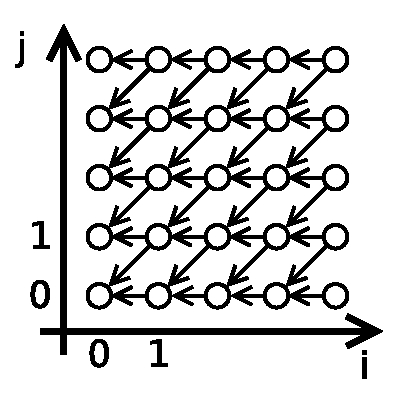
\includegraphics[width=0.55\textwidth]{Figures/ExampleLoopNestPolytope2.eps}
    \label{fig:ExampleLoopNestPolytope}
    \end{minipage}
  }
  \caption{An example loop nest with its polyhedral representation}
  \label{fig:ExampleLoopNest}
\end{figure}
\resetlst

\lstset{frame=none}
\begin{figure}[htbp]
  \centering
  \subfloat[Polyhedral representation of the skewed loop nest presented in Figure \ref{lst:ExampleLoopNestTransformed}]{%
    \begin{minipage}[c][4cm]{%
           0.5\textwidth}
           \centering%
    \includegraphics[width=0.85\textwidth]{Figures/ExampleLoopNestPolytopeTransformed2.eps}
    \label{fig:ExampleLoopNestTransformedPolytope}
    \end{minipage}
  }
  \subfloat[Skewed version of the loop nest presented in \ref{lst:ExampleLoopNest} (pseudo C code)]{%
    \begin{minipage}[c][4cm]{%
           0.5\textwidth}
           \centering%
    \lstset{language=C, escapechar=!}
    \lstinputlisting{Primitives/Code/ExampleLoopNestTransformed2.c}
    \label{lst:ExampleLoopNestTransformed}
    \end{minipage}
  } 
  
  %\caption{Skewed version of listing \ref{lst:ExampleLoopNest} with its polyhedral representation}
  \label{fig:ExampleLoopNestTransformed}
%\end{figure}
%\resetlst
\bigskip

%\lstset{frame=none}
%\begin{figure}[htbp]
  \centering
  \subfloat[Figure \ref{lst:ExampleLoopNestTransformed} after tiling]{%
    \begin{minipage}[c]{%
           0.5\textwidth}
           \centering
    \lstset{language=C, escapechar=!}
    \lstinputlisting{Primitives/Code/ExampleLoopNestTransformedTiled2.c}
    \label{lst:ExampleLoopNestTransformedTiled}
    \end{minipage}
  } 
  \subfloat[Vectorized version of Figure \ref{lst:ExampleLoopNestTransformedTiled}]{%
    \begin{minipage}[c]{%
           0.5\textwidth}
           \centering%
    \lstset{language=C, escapechar=!}
    \lstinputlisting{Primitives/Code/ExampleLoopNestTransformedTiledVectorized2.c}
    \label{lst:ExampleLoopNestTransformedTiledVectorized}
    \end{minipage}
  } 
  \caption{Possible optimized versions of Figure \ref{lst:ExampleLoopNest}}
  \label{fig:ExampleLoopNestTransformedVersions}
\end{figure}
\resetlst

\subsection*{Further Reading}
\begin{itemize}
  \item The Polyhedral Model is More Widely Applicable Than You Think (\citet{BPCB10})
  \item Loop Parallelization in the Polytope Model (\citet{Lengauer93loopparallelization})  
  \item  A practical automatic polyhedral parallelizer and locality optimizer (\citet{Bondhugula:2008:PAP:1379022.1375595})
  \item PoCC - The Polyhedral Compiler Collection (\citet{PoCC:Online})
  \item Polyhedral parallelization of binary code (\citet{Pradelle:2012:PPB:2086696.2086718})
  \item Putting Polyhedral Loop Transformations to Work (\citet{BCGST03})
\end{itemize}

\clearpage

\section{Polly - A Polyhedral Optimizer for LLVM}
\label{Polly}
Exploiting parallelism and data-locality in order to balance the workload
and to improve cache locality are the main goals of the Polly research project.
The polyhedral model is used as abstract mathematical representation to get optimal
results for a particular objective. The three-step approach of Polly first detects
maximal loop nests representable in the polyhedral model.
These representations
are analyzed and transformed before they are again converted to code (here LLVM-IR).
In the case of Polly, the code generation is capable of generating thread 
level parallelism and vector instructions. The code regions Polly is interested 
in are called static control parts, or short SCoPs. Such a SCoP is 
the most central entity within Polly and crucial for any kind of argumentation.
%Apart from the
%following descriptions figure \ref{fig:PollyArchitecture} provides an overview
%of the architecture of Polly.



\subsection{Static Control Parts}
\label{SCoPs}
%\begin{wrapfigure}[]{r}{0.15\textwidth}
  %\centering
  %%\vspace*{-5mm}
  %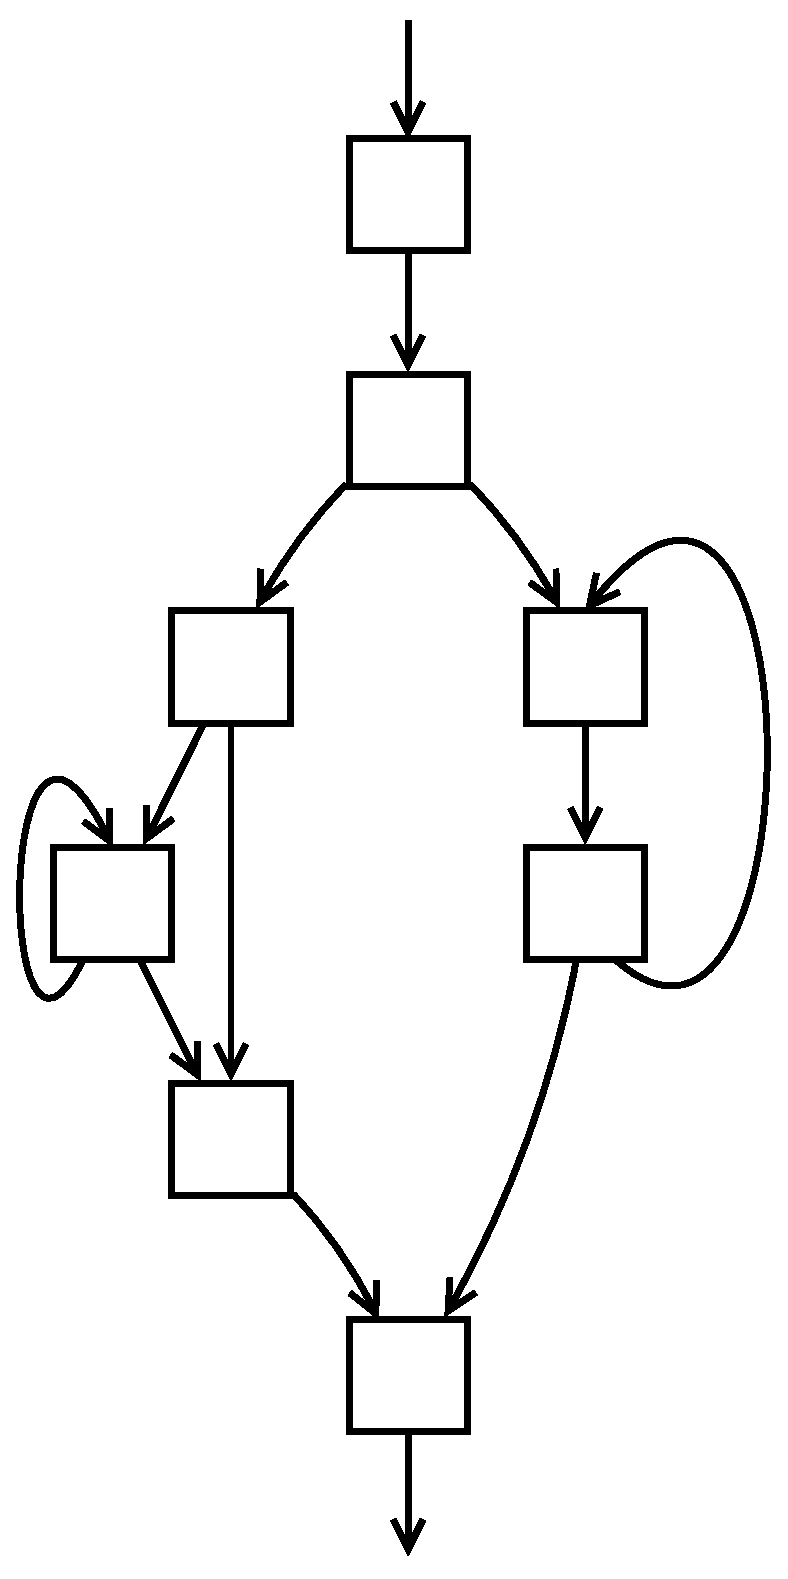
\includegraphics[width=0.15\textwidth]{SimpleRegionCFG.eps}
  %\caption{SCoP CFG}
  %\label{fig:PossibleSCoPCFG}  
%\end{wrapfigure}
A static control part is a region with statically known control flow and memory
accesses. As part of the control flow graph it is restricted to have one entry
edge and one exit edge while loops and conditionals are allowed inside.
To enable precise  prediction of all memory accesses, 
it is necessary to restrict loop bounds and branch 
conditions to be affine expressions with respect to invariant parameters 
and surrounding iteration variables (see definition \ref{def:AffineWithRespect}).
The iteration variables themselves have to
be canonical as stated in definition \ref{def:CanonicalInductionVariable}. 
Because dependencies are crucial for data flow information,
SCoPs are not allowed to contain aliasing pointers at all. 
Furthermore, only affine memory access functions (as described above)
will yield a precise result. Non-affine ones need to be overestimated when they 
are represented in the polyhedral model, but they are not forbidden per se.
The last point concerns called function as only side effect free functions without 
any memory accesses are allowed here. 
%A summary of the  described restrictions and theirs 
%counterparts within the SPolly framework can be found in the appendix.
%Figure \ref{fig:PossibleSCoPCFG} shows the CFG of SCoP 

While the code can be transformed to fulfill some of these conditions 
(e.g., the canonical induction variables), the remaining ones are still 
quite restrictive. The desired results, namely the SCoPs, are valuable because
they can be represented within the polyhedral model. Further analyses and
transformations do not need to deal with the details of the represented code.

Although, all regions fulfilling these requirements are
technically SCoPs, we will restrict ourselves to those containing at least one loop.
The full list of restrictions on SCoPs is given in Table \ref{tab:SCoPRestrictions}.

\begin{table}[htbp] 
  \begin{framed}
  \centering
  \caption{Restrictions on SCoPs}
  \begin{itemize}
      \renewcommand{\labelitemi}{$\triangleright$}
      \item Only simple regions not containing the entry block of the function
      \item Only nested loops and conditionals
      \item Only branches with affine conditions
      \item Only affine accesses based on a constant (base) pointer 
      \item No unsigned iteration variables \footnotemark[1]
      \item No aliasing pointers
      \item Only canonical PHI nodes and induction variables
      \item Instructions may not be used in PHI nodes outside the region\footnotemark[1]
      \item Only ``readnone'' function calls
      \item No alloca or cast instructions within the region
      \item Only affine trip counts for loops
      \item No PHI nodes in the region exit block
      \item \textit{At least one loop contained}
    \end{itemize}
    \flushleft{\footnotemark[1] open for further work }
  \label{tab:SCoPRestrictions}
  \end{framed}
\end{table}

~\\
\begin{definition}[Affine Transformation] ~\\
  Affine transformations are linear transformations followed by a translation.
  Thus they can be written as:
  \[ f(x_1,\dots,x_n) := A_1\, x_1 + \dots + A_n\, x_n + b\]

  \label{def:AffineTransformation}
\end{definition}

\begin{definition}[Affine Expressions] ~\\
  An expression is called affine with respect to a set $X$, when the expression
   can be described as an affine transformation $f$
    (see definition \ref{def:AffineTransformation})
  and the domain of $f$ is restricted to $X$. 
  \label{def:AffineWithRespect}
\end{definition}

\begin{definition}[Canonical Induction Variable] ~\\
  An induction variable is canonical if it starts at zero and steps by one.
  \label{def:CanonicalInductionVariable}
\end{definition}

\subsection{SCoP Detection}
Pollys SCoP detection is the gateway to all further analyses and 
transformations. All regions fulfilling the properties described in the 
last Section, or in short, all (valid) SCoPs are detected here. 
This part is of particular interest because only the accepted regions
will be considered for polyhedral optimizations. 
Almost regardless of its content, any region could be given to
Polly if the SCoP detection is properly instrumented, e.g., by disabling certain 
checks. An important consequence derived from this fact is:
Utilizing the strength of Polly is possible in much more situations than
intentionally implemented, provided that there is a mechanism to deal with 
possibly unsound results.


\subsection{Loop Optimizations}
By default, Polly consults the integer set library (isl) to compute the
final schedule of a SCoP, but alternatively it is possible to use the more 
matured Pluto \cite{Bondhugula07pluto:a}, too. 
Internally isl uses an optimized version of the algorithm 
proposed by Bondhugula et al. \cite{Bondhugula:2008:PAP:1379022.1375595}, which 
is in fact the base algorithm of Pluto. 
Traditional loop optimizations such as blocking, interchange, splitting,
unrolling or unswitching are implicitly applied during this step. 
%Not only the new scheduling but also the new data dependencies are computed, 
%crucial to exploit parallelism.
%Based on these dependencies parallelism is exploited as explained in the next section. 

%\textit{The loop optimizations offers many possibilities in the context 
%of Sambamba (see \ref{FurtherWorkISL}).}


\subsubsection{Parallel Code Generation}
While cache locality is implicitly improved by rescheduling of the loop nest, 
parallel code needs to be generated explicitly afterwards.
Polly is capable of exploiting thread level parallelism using OpenMP \cite{raghesh2011framework}
and data level parallelism using SIMD instructions (called vector instructions here). 
%The former one depends on the OpenMP shared library 
%being present while the later one uses the LLVM built-in vector instruction.
If the former one is desired, the first loop without any loop carried 
dependencies will be rewritten as if there were OpenMP annotations in the first
place. Enabling the latter one, namely vector code generation, 
will not only try to vectorize the innermost loop but also change the  
scheduling process in order to allow this in more cases.

%\begin{figure}[htbp]
  %\centering
  %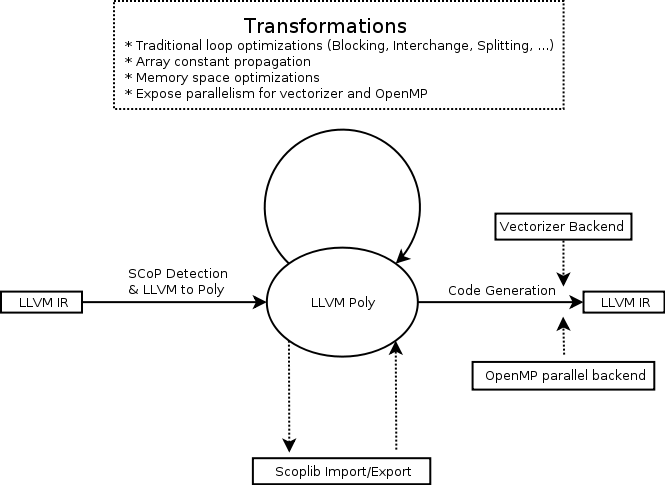
\includegraphics[width=0.9\textwidth]{architecture.png}
  %\caption{Pollys architecture \cite{Polly:Online}}
  %\label{fig:PollyArchitecture}  
%\end{figure}


\subsection*{Further Reading}

\begin{itemize}
  \item Enabling Polyhedral Optimizations in LLVM (\citet{grosser:thesis})
  \item Polly - Polyhedral optimization in LLVM (\citet{grosser.11.impact})  
  %\item A Framework for Automatic OpenMP Code Generation \cite{raghesh2011framework}
  \item Base algorithm of isl (\citet{Bondhugula:2008:PAP:1379022.1375595})
  \item \url{http://polly.llvm.org} \nocite{Polly:Online}
  \item \url{http://www.kotnet.org/~skimo/isl/} \nocite{ISL:Online}
\end{itemize}





\clearpage
\section[Sambamba - A Framework for Adaptive Program Optimization]{Sambamba - \\ A Framework for Adaptive Program Optimization}
%The Sambamba project is built on top of the LLVM compiler infrastructure and 
%aims at adaptive and speculative runtime optimizations.
%Dynamic information about arguments or the global state may allow optimization
%which could not be applied at compile 
%\begin{wrapfigure}[]{r}{0.3\textwidth}
  %\centering
  %%\vspace*{-5mm}
  %\includegraphics[width=0.3\textwidth]{SambambaConcept.eps}
  %\caption{Sambamba in a nutshell}
  %\label{fig:SambambaConcept}  
%\end{wrapfigure}
%time or did not seem interesting back then. It is easily extendible with 
%compile time and a runtime parts. While each one is conceptually 
%independent, the compile time parts may store information which can be accessed
%at runtime to reduce the overhead, even if expensive analysis results are needed. 
%Another fundamental pillar of the framework is the multi versioning system which
%allows for different, specialized function versions.
%[TODO FILL THIS PAGE ]
%%[TODO should VMAD be mentioned here]
%%A similar approach has
%%been published by Jimborean et al.\cite{JIMBOREAN-2012-664345}, in fact th
%%In both cases a dispatcher is used to choose one of the available 
%%implementations each time the function is called. 
%%In this manner exclusive optimizations can be applied on the same function and
%%according to the input a version can be dispatched. Runtime profiling also 
%%reveals opportunities to speculatively transform the program and obtain more
%%specialized versions. A main difference between Sambamba and the work of 
%%Jimborean is probably how these function versions are constructed. Sambamba does
%%not rely on source code annotations but allows all modules to find and extract
%%the versions fully automatic. 
%A high level view on the Sambamba concept is given
%by figure \ref{fig:SambambaConcept} before some of the  built-in utilities 
%and modules, used during this work, are explained. 
\begin{wrapfigure}{r}{0.4\textwidth}
  %\vspace*{-4mm}
  \centering
  \includegraphics[width=0.4\textwidth]{SambambaConcept.eps}
  \caption{Conceptual stages in the Sambamba framework}
  \label{fig:SambambaConcept}
  %\vspace{-4mm}
\end{wrapfigure}
The Sambamba project is built on top of the LLVM compiler infrastructure and 
aims at adaptive and speculative runtime optimizations.
It is easily extensible by modules consisting of a
compile time and a runtime part. 
While they are conceptually independent,
the compile time parts may store information which can be later on accessed
by the runtime part. Apart from this ``data store'', Sambamba offers a way to 
maintain several (semantically equivalent) variants of a function. As there might be 
no order of any kind between those variants, it is admissible to think of them 
as somehow specialized versions. This method versioning allows to store 
conservatively and speculatively optimized versions in order to switched between 
them during runtime. 
%But both can profit from specialization at runtime. 
%especially after conflicting speculation.
%Based on the LLVM suite, Sambamba uses the shipped JIT compiler 
%and a software transactional memory system to secure
%speculative execution. 
%In the context of speculation and profiling, Sambamba can be used to store
%several version of a method which can be generated by one of the two parts.
Profiling combined with the method versioning system allows runtime interactions
to explore more parallelism or minimize the overhead in case of misspeculation. 

\paragraph{Stages in the Sambamba framework}~\\ 
As illustrated in Figure \ref{fig:SambambaConcept} we can differentiate five 
conceptual stages embedded in the Sambamba framework.

{\begin{list}{}
    {\setlength{\leftmargin}{-0mm}}
  \item[]
\begin{enumerate}
  \item[\textbf{[A]}] Execute static whole-program \textbf{analyses}  
  with the possibility to save their results.
\item[\textbf{[P]}] Speculatively \textbf{parallelize} parts of the program
  based on the results of \textbf{[A]} and \textbf{[S]}.
\item[\textbf{[X]}] Detect and recover from conflicts by speculative
  \textbf{execution} using a software transactional memory system (see next Section).
\item[\textbf{[C]}] Use the profiles and misspeculation information gained 
  during the execution to \textbf{calibrate} future optimization steps.
\item[\textbf{[S]}] Generate \textbf{specialized} variants of a function, 
 one for each special input profile detect by \textbf{[C]}. 
\end{enumerate}
\end{list}
}


\subsection{Software Transactional Memory}
A software transactional memory system (STM) is a conflict management system used to detect
memory conflicts in speculatively parallelized programs and closely related to
the transaction system in databases. When in use, the STM logs
all accesses to the memory within a certain code region.
If, during the execution of this region, a memory address has been accessed
by different threads and at least one of them was a writing one, all reading
ones (during the concurrent execution and later on) may read illegal data.
As a consequence, all resulting computations might be wrong. Such cases will be
detected by the STM and  conflicting threads might be forced to recompute 
their results. These recomputations are also called  rollbacks.
Different STM implementations will, for example,
allow at least one thread to finish its computation before all the others might
have to recompute theirs. Such implementations will maintain the liveness of
a system. 
%even though the
%required execution time might be quadratic in the number of threads.

%\paragraph{Extensions} ~\\
As the described implementation only preserves liveness but no order between
the different computations, there is an extension called commit order. 
A commit is the final synchronization step of a thread in an STM environment and
a commit order will enforce the threads to synchronize, thus store their result
permanently, in a determined order. For later argumentation we will assume the 
creation order of the threads. 
Just like the unordered version this one maintains liveness because there is always
one thread at the front of the remaining ones. 

Another possible extension for an STM system is a wait construct which is built
on top of the commit order. Such a wait will cause the thread to pause until 
all preceding threads (in the commit order) have successfully committed their results.
The section from the wait construct to the commit point forms a mutual exclusive
area which can only be entered by one thread at a time and only if the preceding
ones have been already successfully synchronized. Furthermore, the wait can only
be passed by a thread if there is no conflict with all previous commits, otherwise
the computation starts again at the beginning. Together, this guarantees that a 
thread passing the wait construct is able to successfully commit its results, in 
fact this thread will be the next committing one.

The current STM implementation in the Sambamba framework does neither provide a 
commit order nor the wait construct, but this will change in the near future.


\clearpage

\subsection{Parallel Control Flow Graphs}
\begin{wrapfigure}[]{r}{0.43\textwidth}
  \centering
  %\vspace*{-3mm}
  \begin{minipage}[c][0.43\width]{\textwidth}
  \begin{tabular}{c}
  \includegraphics[width=0.38\textwidth]{ParallelSectionEx.eps}
  \end{tabular}
  \end{minipage}
  \caption{A parallel section with three transactions (colored regions)}
  %\vspace*{-3mm}
  \label{fig:ParallelSectionEx}  
\end{wrapfigure}
A parallel control flow graph (ParCFG) is a data structure used by the
Sambamba parallelizer module to express parallel sections within an ordinary CFG. 
Each parallel section consists of an entry block called \texttt{piStart} and
an exit block called \texttt{piEnd}.
The \texttt{piStart} has an arbitrary number of successors, each denotes a
(concurrent) transaction possibly guarded by the STM. All transactions end in the 
\texttt{piEnd} block after some arbitrary computation. 
To put it in another way, parallel sections represent 
fork-join parallelism where the \texttt{piStart} block forks transactions 
which are synchronized (or commited) at the corresponding \texttt{piEnd} block. 
%In the case of Sambamba this
%synchronization is done by a software transaction memory as described in the 
%next section.

Figure \ref{fig:ParallelSectionEx} shows such a parallel section with three 
highlighted transactions. 
%At runtime they will be executed concurrently, each 
%by one worker thread at a time.
%\\

\subsection{The Sambamba Parallelizer}
\begin{wrapfigure}[]{l}{0.40\textwidth}
  \centering
  \vspace*{-0mm}
  \includegraphics[width=0.38\textwidth]{TransactionQueue.eps}
  \caption{Illustration of the transaction queue with three worker threads}
  %\vspace*{-4mm}
  \label{fig:TransactionQueue}  
\end{wrapfigure}
The Sambamba parallelizer will become the main interface for any kind of 
parallelization in the framework. At the moment, it is in need of parallel control
flow graphs to explicitly state section which should be executed in parallel, but
in the future an automatic loop parallelization component will be implemented too. 
The runtime part of the parallelizer instantiates as many worker threads as 
there are cores on the executing machine. Each worker thread will later on execute 
one transaction at a time. In contrast to the OpenMP approach
no external libraries are needed to exploit parallelism. 

Figure \ref{fig:TransactionQueue} presents a stylized transaction queue which is
currently used to distribute the work among the worker threads. 

Note that there is a new parallelizer module implemented by now which utilizes
the ``Intel(R) Threading Building Blocks'' (TBB) framework \cite{Corporation_2008}. 
As the evaluation of this work used the ``old'' implementation, the 
description given above might not fit the current state of Sambamba.

\subsection*{Further Reading}
\begin{itemize}
  \item Sambamba: A Runtime System for Online Adaptive Parallelization (\citet{DBLP:conf/cc/StreitHZH12})
  \item \url{http://www.sambamba.org} 
\end{itemize}



